\documentclass[../main.tex]{subfiles}
\graphicspath{{\subfix{../figures/}}}
%
\begin{document}
\section{工厂方法模式}
工厂方法模式(Factory Method)是类形式的创建模式,又叫做虚拟构造器(Virtual Constructor)模式或者多态性工厂(Polymorphic Factory)模式。
工厂方法模式将定义一个创建产品对象的工厂接口,将实际创建功能放到具体工厂子类中。

\textbf{简单工厂模式的优缺点}:
在简单工厂模式中,一个工厂类处于对产品类实例化的中心位置上,它知道每一个产品,它决定哪一个产品类应当被实例化。这个模式的优点是允许客户端相对独立于产品创建的过程,并且在系统引入新产品的时候无需修改客户端,也就是说,它在某种程度上支持开闭原则。
这个模式的缺点是对开闭原则的支持不够,因为如果有新的产品加入到系统中去,就需要修改工厂类,将必要的逻辑加入到工厂类中。

\textbf{平行的等级结构}:在一个系统设计中,常常是首先有产品角色,然后有工厂角色。在可以应用工厂方法模式的情形下,一般都会有一个产品的等级结构,其由一个(甚至多个)抽象产品和多个具体产品组成。产品的等级结构如下图所示,树图中有阴影的是树枝型节点。
\begin{figure}[H]
  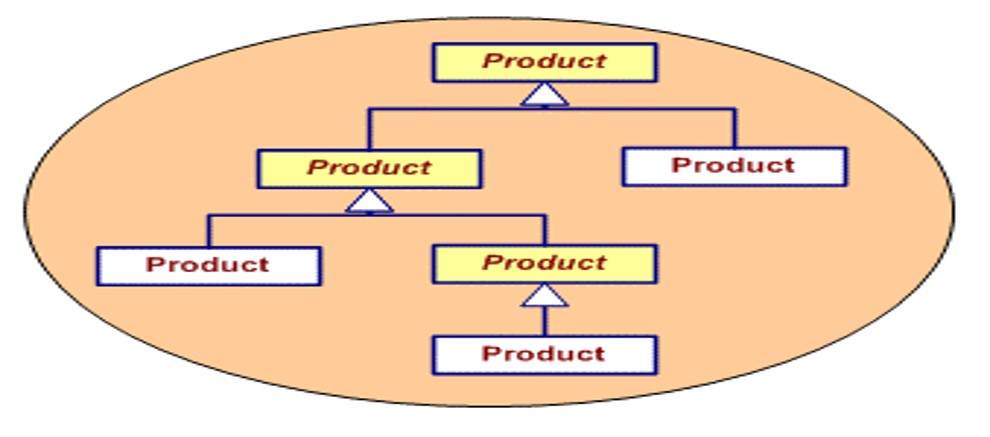
\includegraphics[width=0.45\textwidth]{16_1.jpg}
\end{figure}
在上面的产品等级结构中,出现了多于一个的抽象产品类,以及多于两个的层次。这其实是真实的系统中常常出现的情况。
当将工厂方法模式应用到这个系统中去的时候,常常采用的一个做法是按照产品的等级结构设计一个同结构的工厂等级结构。工厂的等级结构如下图所示,树图中有阴影的是树枝型节点。
\begin{figure}[H]
  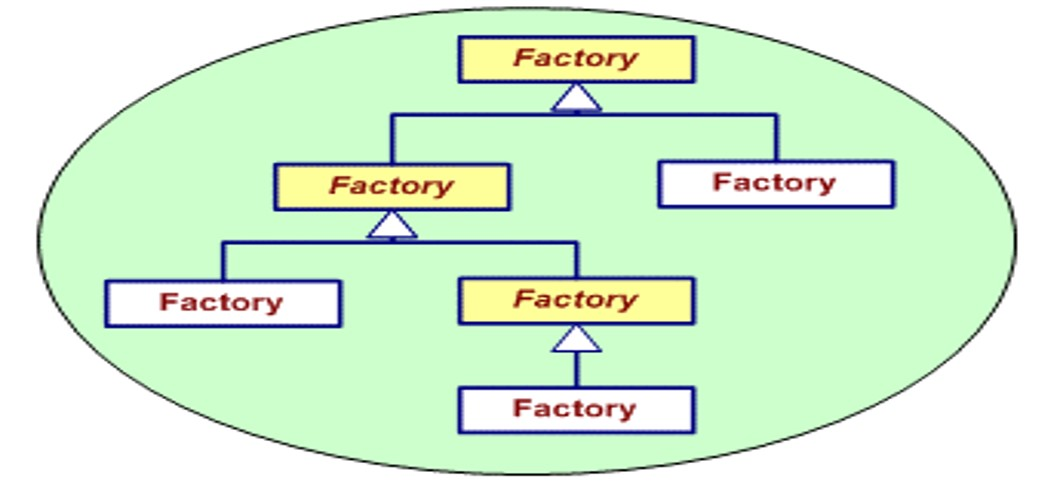
\includegraphics[width=0.45\textwidth]{16_2.jpg}
\end{figure}
然后由相应的工厂角色创建相应的产品角色,工厂方法模式的应用如下图所示,图中的虚线代表创建(依赖)关系。
工厂方法模式并没有限制产品等级结构的层数。
\begin{figure}[H]
  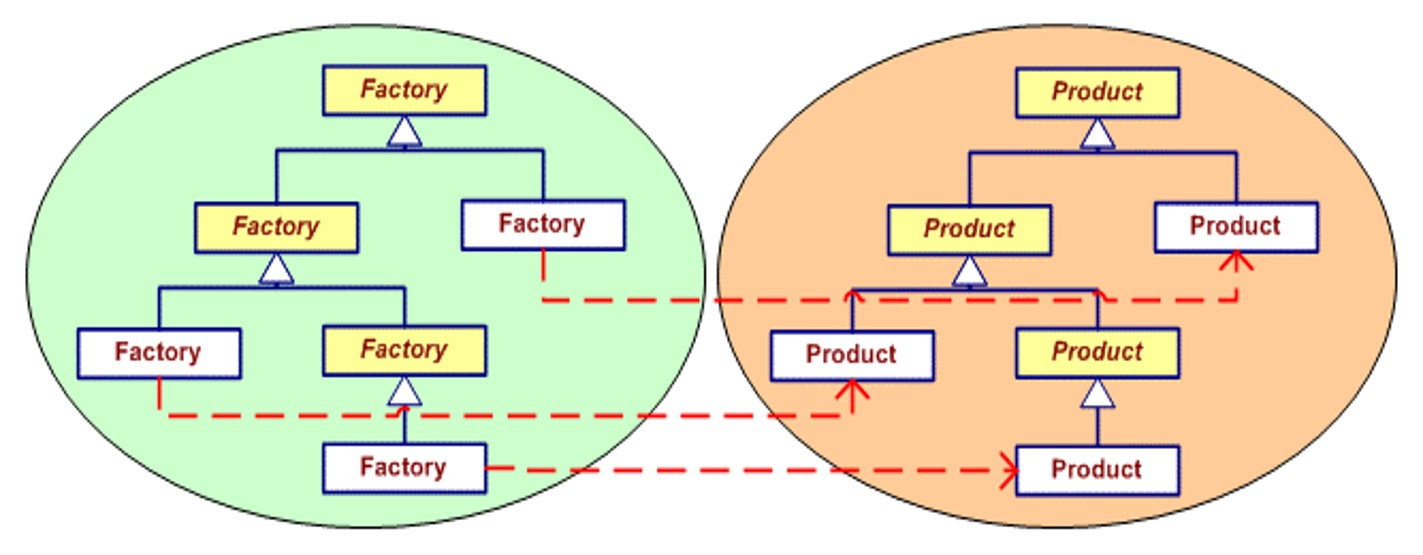
\includegraphics[width=0.45\textwidth]{16_3.jpg}
\end{figure}
%
\subsection{工厂方法模式的结构}
\noindent 为说明工厂方法模式的结构,下面以最简单的情形为例。此示意性系统类图如下所示。
%
\begin{figure}[H]
  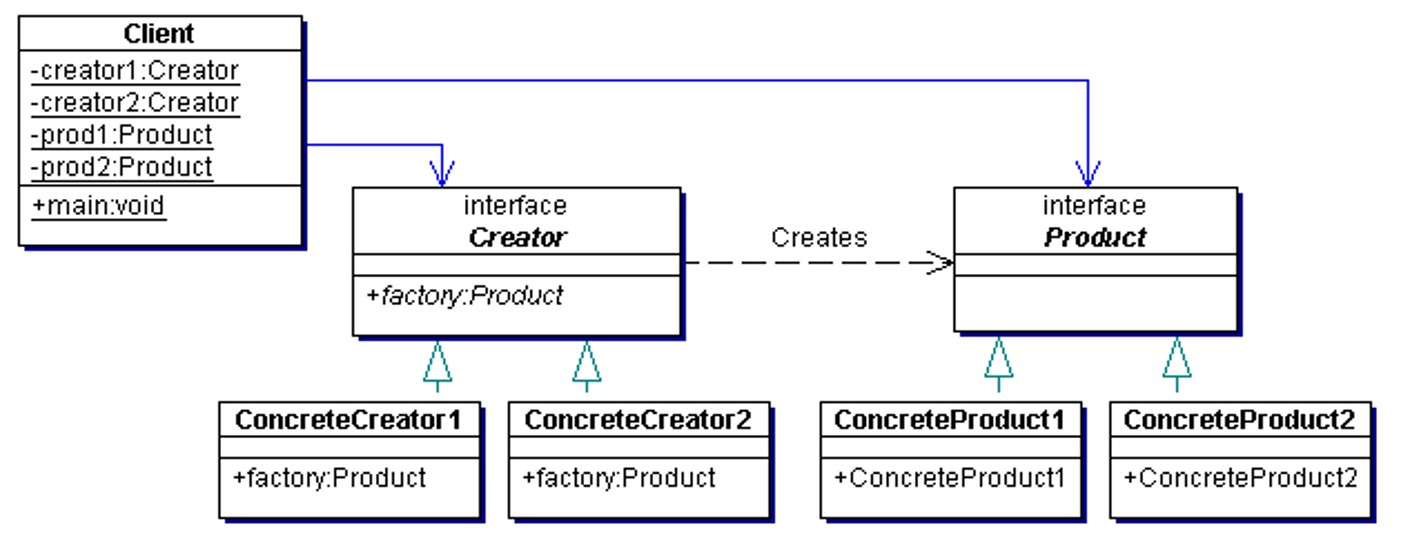
\includegraphics[width=0.55\textwidth]{16_4.jpg}
\end{figure}
%
从上图可以看出,这个使用了工厂方法模式的系统涉及到以下的角色:
\begin{itemize}
  \item 抽象工厂(Creator)角色:担任这个角色的是工厂方法模式的核心,它是应用无关的。任何在模式中创建对象的工厂类必须实现这个接口。在上面的系统中这个角色由Java 接口Creator 扮演;在实际的系统中,这个角色也常常使用抽象Java 类实现。
  \item 具体工厂(Concrete Creator)角色:担任这个角色的是实现了抽象工厂接口的具体Java 类。具体工厂角色含有与应用密切相关的逻辑,并且受到应用程序的调用以创建产品对象。在本系统中给出了两个这样的角色,也就是具体Java 类ConcreteCreator1 和ConcreteCreator2。
  \item 抽象产品(Product)角色:工厂方法模式所创建的对象的超类型,也就是产品对象的共同父类或共同拥有的接口。在本系统中,这个角色由Java 接口Product 扮演;在实际的系统中,这个角色也常常使用抽象Java 类实现。
  \item 具体产品(Concrete Product)角色:这个角色实现了抽象产品角色所声明的接口。工厂方法模式所创建的每一个对象都是某个具体产品角色的实例。
  \item 客户端(Client)角色:为了说明这个系统的使用办法,特地引进了一个客户端角色Client。这个角色创建工厂对象,然后调用工厂对象的工厂方法创建相应的产品对象。
\end{itemize}
%
\begin{lstlisting}[language=java]
public interface Creator {
  // 工厂方法
  public Product factory();
}

public interface Product {  }

public class ConcreteCreator1 implements Creator {
  // 工厂方法
  public Product factory() { return new ConcreteProduct1(); }
}

public class ConcreteProduct1 implements Product {
  public ConcreteProduct1() {
    // do something
  }
}

public class Client {
  private static Creator creator1, creator2;
  private static Product prod1, prod2;
  public static void main(String[] args) {
    creator1 = new ConcreteCreator1();
    prod1 = creator1.factory();
    creator2 = new ConcreteCreator2();
    prod2 = creator2.factory();
  }
}
\end{lstlisting}
工厂方法模式的活动序列图:
\begin{figure}[H]
  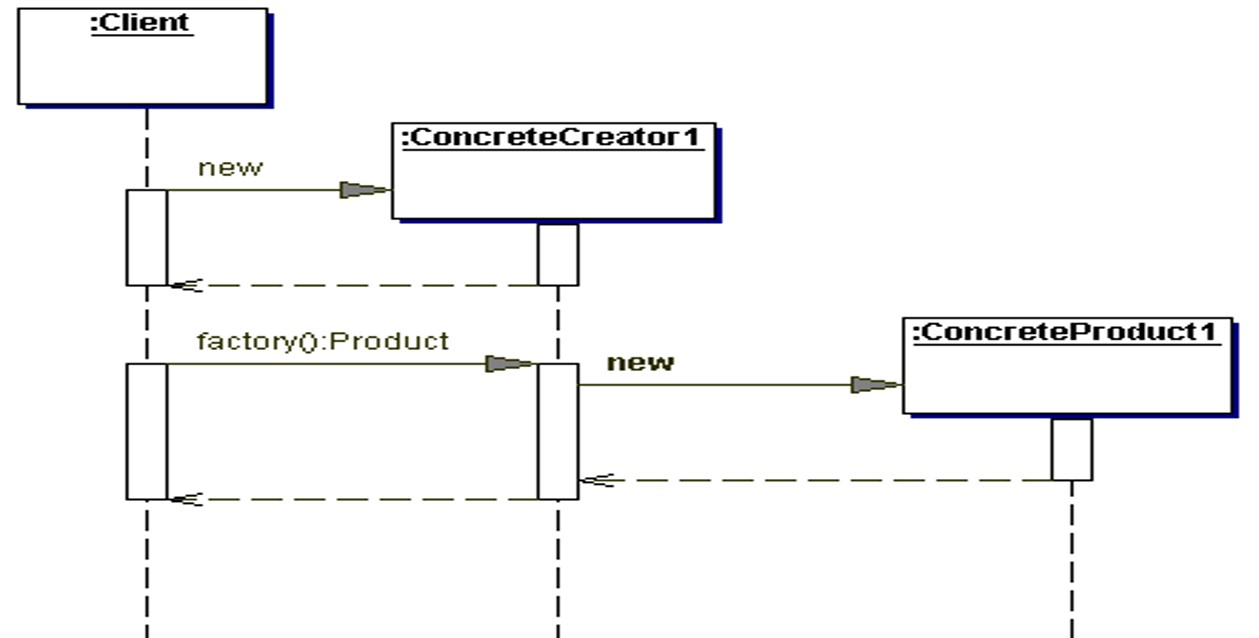
\includegraphics[width=0.55\textwidth]{16_5.jpg}
\end{figure}
Client 对象的活动可以分成两部分。
\begin{enumerate}
  \item 客户端创建ConcreteCreator1 对象。这时客户端所持有变量的静态类型是Creator,而实际类型是ConcreteCreator1。然后,客户端调用ConcreteCreator1 对象的工厂方法factory(),接着后者调用ConcreteProduct1 的构造子创建出产品对象。
  \item 客户端创建一个ConcreteCreator2 对象,然后调用ConcreteCreator2 对象的工厂方法factory(),而后者调用ConcreteProduct2 的构造子创建出产品对象.
\end{enumerate}
%
\textbf{工厂方法模式和简单工厂模式}:工厂方法模式和简单工厂模式在结构上的不同是很明显的。工厂方法模式的核心是一个抽象工厂类,而简单工厂模式把核心放在一个具体类上。工厂方法模式可以允许很多具体工厂类从抽象工厂类中将创建行为继承下来,从而可以成为多个简单工厂模式的综合,进而推广了简单工厂模式。
工厂方法模式退化后可以变得很像简单工厂模式。设想如果非常确定一个系统只需要一个具体工厂类,那么就不妨把抽象工厂类合并到具体的工厂类中去。由于反正只有一个具体工厂类,所以不妨将工厂方法改成为静态方法,这时候就得到了简单工厂模式。

工厂方法模式之所以有一个别名叫\textbf{多态性工厂模式},显然是因为具体工厂类都有共同的接口,或者都有共同的抽象父类。
如果系统需要加入一个新的产品,那么所需要的就是向系统中加入一个这个产品类以及它所对应的工厂类。没有必要修改客户端,也没有必要修改抽象工厂角色或者其他已有的具体工厂角色。对于增加新的产品类而言,这个系统\textbf{完全支持开闭原则}。

\textbf{Java 语言中工厂方法模式的例子}:在Java 聚集中的应用,
Java 聚集是Java1.2 版提出来的。多个对象聚在一起形成的总体称之为聚集(Aggregate),聚集对象是能够包容一组对象的容器对象。所有的Java 聚集都实现java.util.Collection 接口,这个接口规定所有的Java 聚集必须提供一个iterator()方法,返还一个Iterator (迭代器:first();next();)类型的对象,如下图所示。
一个具体的Java 聚集对象会通过这个iterator()方法接口返还一个具体的Iterator 类。可以看出,这个iterator()方法就是一个工厂方法。
\begin{figure}[H]
  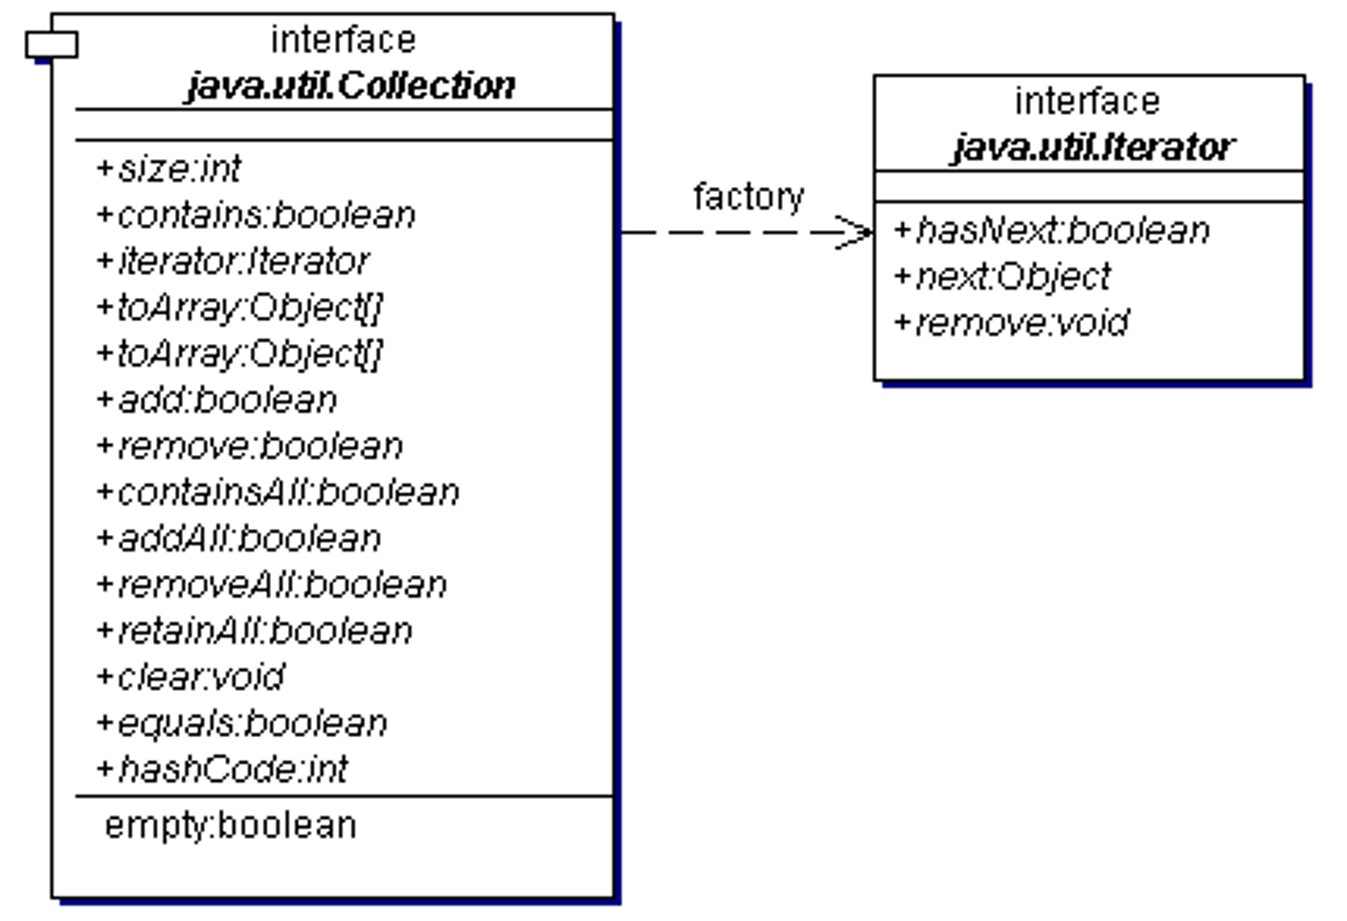
\includegraphics[width=0.65\textwidth]{16_6.jpg}
\end{figure}
%
\subsection{工厂方法模式在农场系统中的实现}
\noindent 取代了过去的全能角色的是一个抽象的园丁角色,这个角色规定出具体园丁角色需要实现的具体职能,而真正负责作物管理的则是负责各种作物的具体园丁角色。
此处仍然考虑前面所讨论过的植物,包括葡萄(Grape)、草莓(Strawberry)以及苹果(Apple)等。专业化的管理要求将有专门的园丁负责专门的水果,比如苹果由苹果园丁负责,
草莓有草莓园丁负责,而葡萄由葡萄园丁负责。这些苹果园丁、草莓园丁以及葡萄园丁都是实现了抽象的水果园丁接口的具体工厂类,而水果园丁则扮演抽象工厂角色。

\noindent 多态农场系统的设计图就如下图所示。
抽象工厂类 FruitGardener 是工厂方法模式的核心,但是它并不负责具体水果或蔬菜的种植。相反地,这项权力被交给子类,即 AppleGardener StawberryGardener 以及 GrapeGardener。
\begin{figure}[H]
  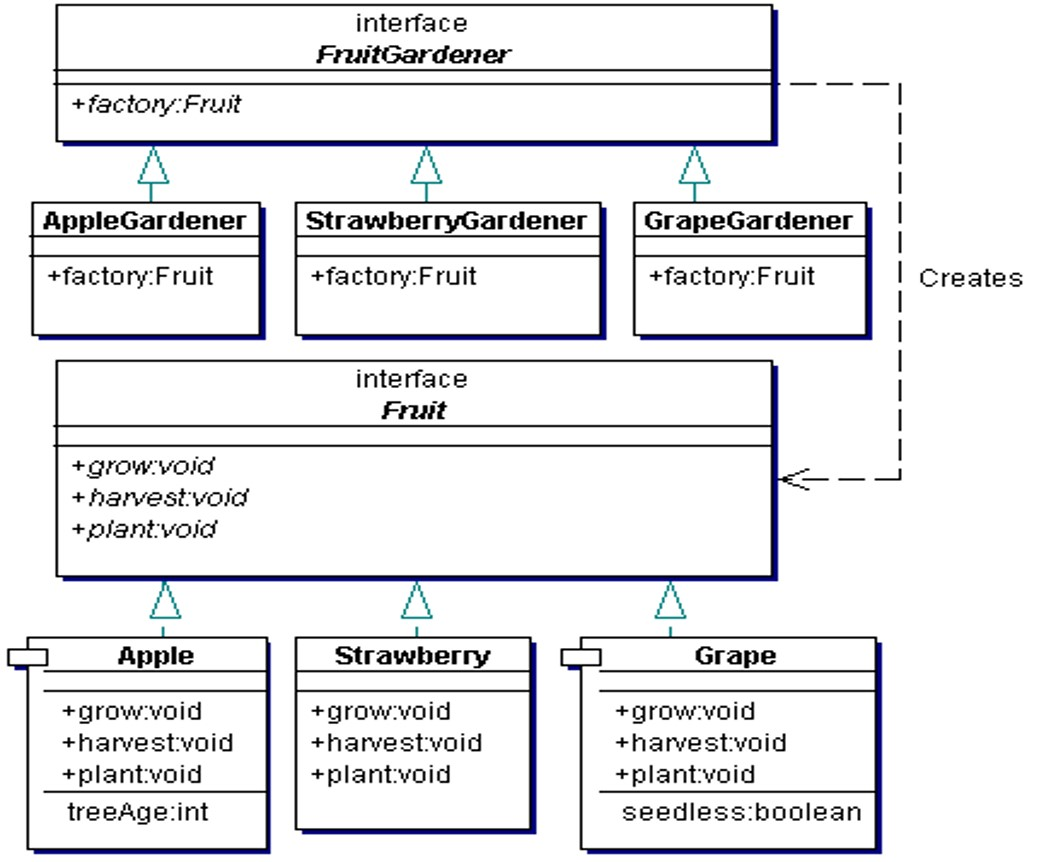
\includegraphics[width=0.65\textwidth]{16_7.jpg}
\end{figure}
%
\begin{lstlisting}[language=java]
// 抽象工厂角色
public interface FruitGardener {
  // 工厂方法
  public Fruit factory();
}

public class AppleGardener implements FruitGardener {
  // 工厂方法
   public Fruit factory() {
     return new Apple();
   }
}

public class StrawberryGardener implements FruitGardener {
  // 工厂方法
  public Fruit factory() {
    return new Strawberry ();
  }
}

public class GrapeGardener  implements FruitGardener {
  // 工厂方法
  public Fruit factory() {
    return new Grape ();
  }
}

public interface Fruit {
  abstract void grow();
  abstract void harvest();
  abstract void plant();
}

public class Apple implements Fruit {
  private int treeAge;
  public void grow() {
    System.out.println("Apple is growing...");
  }
  public void harvest() {
    System.out.println("Apple has been harvested.");
  }
  public void plant() {
    System.out.println("Apple has been planted.");
  }
  public int getTreeAge() {   return treeAge; }
  public void setTreeAge(int treeAge) { this.treeAge = treeAge; }
}
\end{lstlisting}
\end{document}
